%!TEX root = ../Chapter3.tex
\section{Numerical Illustrations}\label{sec:t3c.experiments}

\subsection{Computation of the optimal error decay rate}\label{sec:t3c.experiments.rate}

We first describe how to approximate $\Gamma_{\beta}^\star$ under any prior of 1-dimensional exponential family. We then also provide a way to compute numerically $\Gamma_{\beta}^\star$ under Gaussian prior since it can be computed more explicitly.

\paragraph{General case.}
For any $i\neq I^\star$, $C_i(\beta,\omega_i)$ is defined as the output to a convex minimization problem for whom the unique solution has an analytic expression
\[
    \frac{\beta}{\beta+\omega_i}\mu_{I^\star} + \frac{\omega_i}{\beta+\omega_i}\mu_i.
\]
Next, we define for any $i\neq I^\star$, a function
\begin{align*}
  g_i \colon [0,+\infty[ &\to [0,+\infty[\\
  x &\mapsto \beta d\left(\mu_{I^\star};\frac{\beta}{\beta+\omega_i}\mu_{I^\star} + \frac{\omega_i}{\beta+\omega_i}\mu_i\right) + x d\left(\mu_i;\frac{\beta}{\beta+\omega_i}\mu_{I^\star} + \frac{\omega_i}{\beta+\omega_i}\mu_i\right).
\end{align*}
In fact, $g_i$ is a strictly increasing function (see~\citealt{garivier2016tracknstop}, Appendix A.2 for more details), so does its inverse function $x_i \eqdef g_i^{-1}$ which is defined on $[0, \beta d(\mu_{I^\star};\mu_i)[$ as $g_i$ tends to 0 when $x$ tends to 0 and tends to $\beta d(\mu_{I^\star};\mu_i)$ when $x$ tends to $+\infty$.

According to Proposition~\ref{prop:optim}, the optimal proportion vector $\bomega^\beta$ that we are searching for satisfies the constraint that $\forall i,j\neq I^\star$,
\[
    g_i(\omega_i^\beta) = g_j(\omega_j^\beta) = \Gamma_{\beta}^\star.
\]
Since $\omega_i^\beta = g_i^{-1}(\Gamma_{\beta}^\star) = x_i(\Gamma_{\beta}^\star)$, and we know that $\sum_{i\neq I^\star} \omega_i = 1-\beta$, thus the problem of computing $\Gamma_{\beta}^\star$ is equivalent to solve the following equation,
\[
    \sum_{i\neq I^\star} x_i(y) = 1 - \beta.
\]
This equation has a unique solution since $\sum_{i\neq I^\star}$ is a strictly increasing function valued in $[0, +\infty[$. We can thus apply a bisection method to this function whose evaluation require itself a bisection method applied on $K-1$ smooth scalar functions.

\paragraph{Gaussian case.}
In the context of this paper, we can do a more efficient approximation. In the Gaussian case, we know that for any $i,j\neq I^\star$,
\[
    \frac{1}{\omega_j^\beta} + \frac{1}{\beta} = \frac{(\mu_{I^\star}-\mu_j)^2}{(\mu_{I^\star}-\mu_i)^2}\left(\frac{1}{\omega_i^\beta} + \frac{1}{\beta}\right).
\]
Denote $x_i\eqdef 1/\omega_i^\beta+1/\beta$ and $a_{ji}\eqdef (\mu_{I^\star}-\mu_j)^2/(\mu_{I^\star}-\mu_i)^2$, fix some $i\neq I^\star$, then we have $\forall j\neq I^\star$, $x_j = a_{ji}x_i$. Since $\sum_{j\neq I^\star} \omega_j^\beta = 1-\beta$, we have
\[
    \sum_{j\neq I^\star} \frac{1}{x_j-1/\beta} = \sum_{j\neq I^\star} \frac{1}{a_{ji}x_i-1/\beta} = 1-\beta.
\]
Thus we only need to find the unique solution to the equation
\[
    \sum_{j\neq I^\star} \frac{a_{ij}}{x-a_{ij}/\beta} = 1-\beta,
\]
that requires only one shot bisection method.

\subsection{Empirical vs. theoretical sample complexity}\label{sec:t3c.experiments.illustrations}

%\emilie{This appendix could be called ``Rebuttal'' as it is. I would remove it. I already added a few line on ``the importance of randomization'' in the main text. We can see if Figure 3 also fits in the experimental section. If it doesn't, we can add a very early appendix ``Further numerical illustration'' or something like that explaining Figure 3. This appendix has to be referred to in the main text}
%
%\paragraph{The importance of randomization}
%The randomization in Line 3 of Algorithm~\ref{alg:sampling_rule} is essential, without which the algorithm may actually never stop on certain instances. One example is to just set $I^{(1)}$ as the current best arm and run exploration only through Lines 8-14 (that we refer to as \texttt{BC2}). It is actually very close to the “modified Best Challenger (\BC)” algorithm introduced in Section~\ref{sec:experiments}. The difference is that \BC adds some forced exploration, which is replaced by randomization in \TCC (which can be seen as adaptive exploration), as discussed in the 3rd paragraph of Section~\ref{sec:experiments}.
%
%The intuition for the necessity of forced exploration or randomization is the following. On an instance with two sub-optimal arms of the same mean, there is a chance that the algorithm ends up alternating forever between those two arms, and thus would not stop. The randomization prevents it to stay in this trap. To illustrate that this actually happens, we empirically compared \texttt{BC2} to \TCC on a simple problem with three Bernoulli arms (resp. Gaussian arms with variance 1) of means 0.5, 0.4 and 0.4, with the confidence level delta set to 0.01. We set a threshold of $10^7$ samples above which we consider that the algorithm did not stop. Results reported below are averaged over 1000 independent trials. We can see that \texttt{BC2} has higher rate of error and does have a much larger elapsed time compared to \TCC since it did not stop on some of the instances.
%
%\begin{itemize}
%    \item Beta-Bernoulli
%    \begin{itemize}
%        \item \texttt{BC2}
%        \begin{itemize}
%            \item proportion of runs that did not terminate: 0.048
%            \item average number of draws: 32442.55
%            \item proportion of errors: 0.050
%            \item elapsed time: 3316.8
%        \end{itemize}
%        \item \TCC
%        \begin{itemize}
%            \item proportion of runs that did not terminate: 0.0
%            \item average number of draws: 2018.07
%            \item proportion of errors: 0.0
%            \item elapsed time: 17.45
%        \end{itemize}
%    \end{itemize}
%    \item Gaussian
%    \begin{itemize}
%        \item \texttt{BC2}
%        \begin{itemize}
%            \item proportion of runs that did not terminate: 0.06
%            \item average number of draws: 162078.29
%            \item proportion of errors: 0.064
%            \item elapsed time: 613.93
%        \end{itemize}
%        \item \TCC
%        \begin{itemize}
%            \item proportion of runs that did not terminate: 0.0
%            \item average number of draws: 8301.15
%            \item proportion of errors: 0.0
%            \item elapsed time: 8.12
%        \end{itemize}
%    \end{itemize}
%\end{itemize}
%
%Fig.~\ref{fig:bc} (left for Bernoulli bandits and right for Gaussian bandits) provides illustrations of the distribution of the number of samples needed before stopping: the average (black dot) is far worse for \texttt{BC2} and the median is not much better.
%
%\begin{figure}[ht]
%    \centering
%    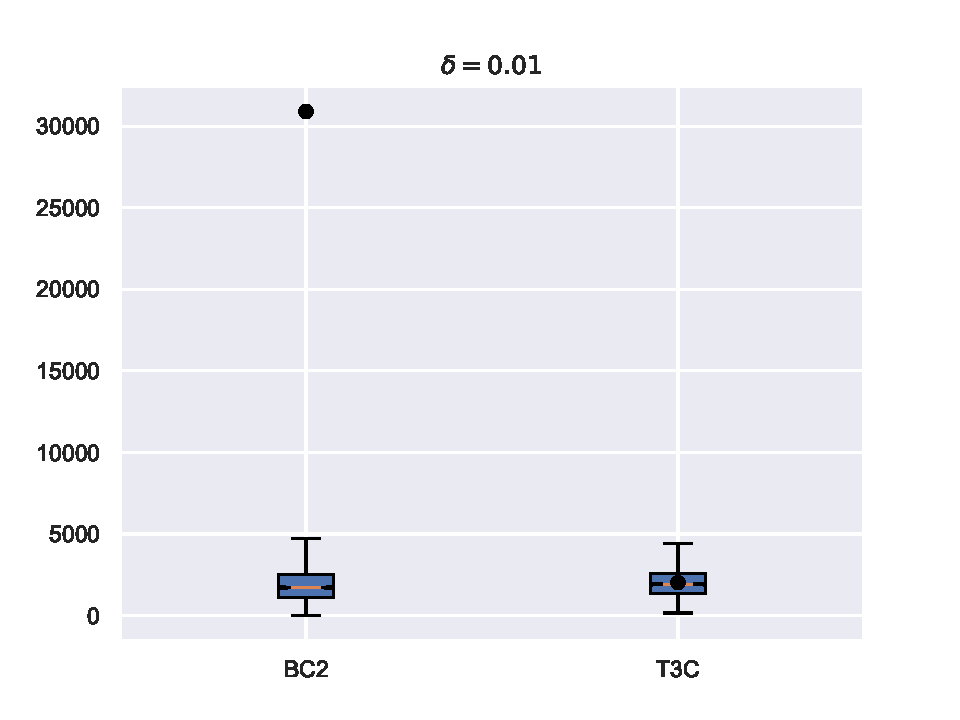
\includegraphics[width=0.49\textwidth]{img/bc2_beta.pdf}
%    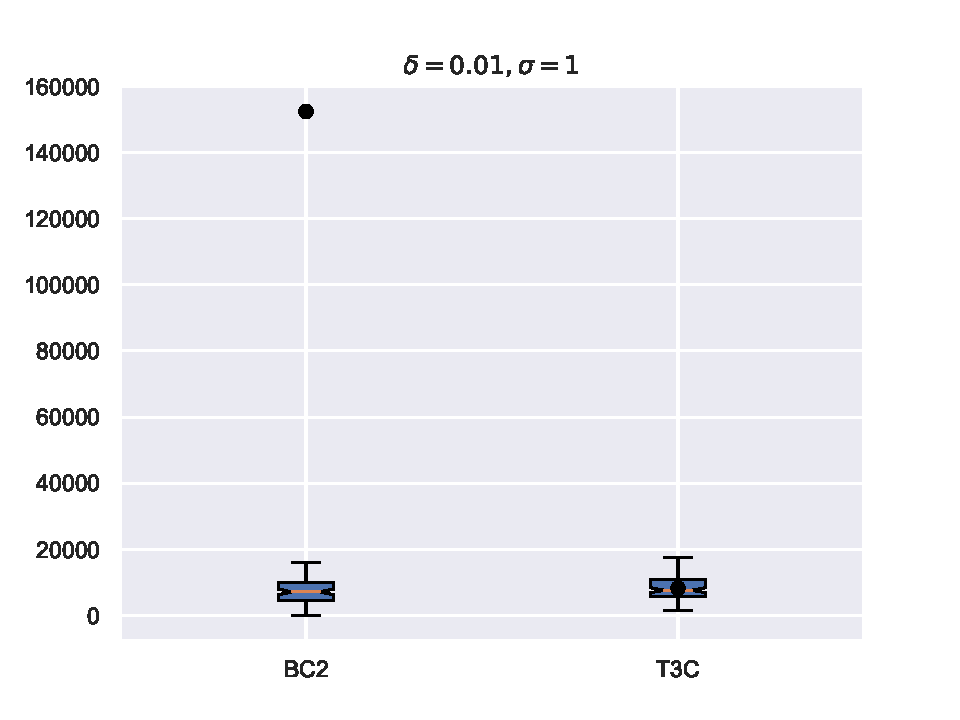
\includegraphics[width=0.49\textwidth]{img/bc2_gaussian.pdf}
%    \caption{why is randomization important.}
%    \label{fig:bc}
%\end{figure}

In Fig.~\ref{fig:t3c.hardness}, we plot expected stopping time of \TCC for $\delta = 0.01$ as a function of $1/\Gamma_\beta^\star$ on 100 randomly generated problem instances. We see on this plot that the empirical stopping time has the right linear scaling in $1/\Gamma_\beta^\star$ (ignoring a few outliers).

\begin{figure}[ht]
    \centering
    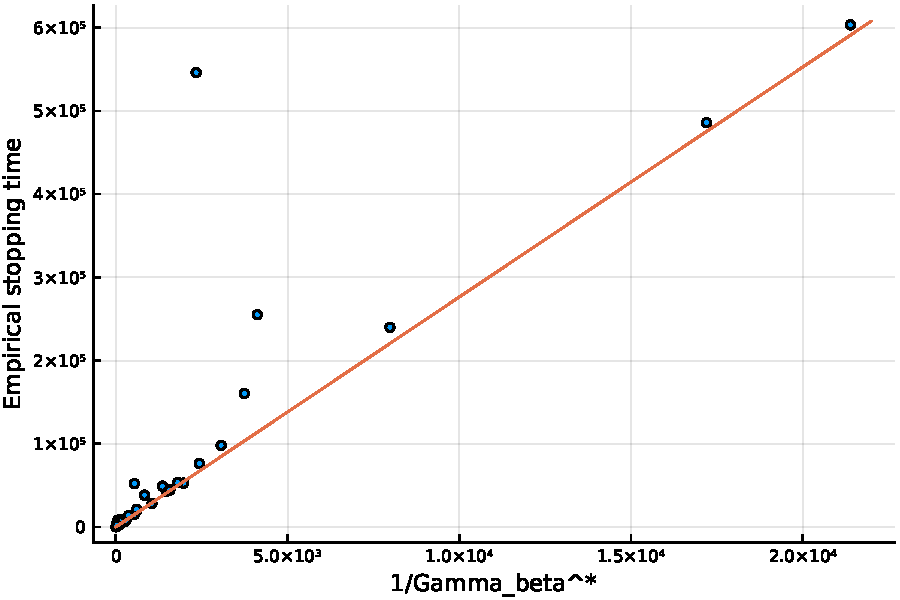
\includegraphics[width=0.49\textwidth]{Chapter3/img/hardness.pdf}
    \caption{dots: empirical sample complexity, solid line: theoretical sample complexity.}
    \label{fig:t3c.hardness}
\end{figure}

\subsection{Results}\label{sec:t3c.experiments.results}
This section is aimed at illustrating our theoretical results and supporting the practical use of Bayesian sampling rules for fixed-confidence BAI.   %We also compare the different sampling rules.
%The main contribution of this paper is theoretical, thus the following experimental results are not for the purpose of showing the superiority of \TCC over existing methods, but rather supports a discussion on sampling rules.

We experiment with three different Bayesian sampling rules: \TCC, \TTTS and \TTEI, and we also include the Direct Tracking (\DT) rule of~\cite{garivier2016tracknstop} (which is adaptive to $\beta$), the \UGapE~\citep{gabillon2012ugape} algorithm, and a uniform baseline. In order to make a fair comparison, we use the Chernoff stopping rule~(\ref{eq:chernoffstoppingtime}) and associated recommendation rule for all of the sampling rules, including the uniform one, except for \UGapE which has its own stopping rule. Furthermore, we include a top-two variant of the Best Challenger (\BC) heuristic (see, e.g., \citealp{menard2019lma}). 

\BC selects the empirical best arm $\hat{I}_n$ with probability $\beta$ and the maximizer of $W_n(\hat{I}_n,j)$ with probability $1-\beta$, but also performs forced exploration (selecting any arm sampled less than $\sqrt{n}$ times at round $n$). \TCC can thus be viewed as a variant of \BC in which no forced exploration is needed to converge to $\bomega^\beta$, due to the noise added by replacing $\hat{I}_n$ with $I_n^{(1)}$.

We consider two simple instances with arms means given by $\bmu_1 = [0.5 \ 0.9 \ 0.4 \ 0.45 \ 0.44999]$, and $\bmu_2 = [1 \ 0.8 \ 0.75 \ 0.7]$ respectively. We run simulations for both Gaussian (with $\sigma=1$) and Bernoulli bandits with a risk parameter $\delta=0.01$. %In the Gaussian case, we set $\sigma=1$.
Figure~\ref{fig:confidence} reports the empirical distribution of $\tau_\delta$ under the different sampling rules, estimated over 1000 independent runs. 

\begin{figure*}[ht]
\centering
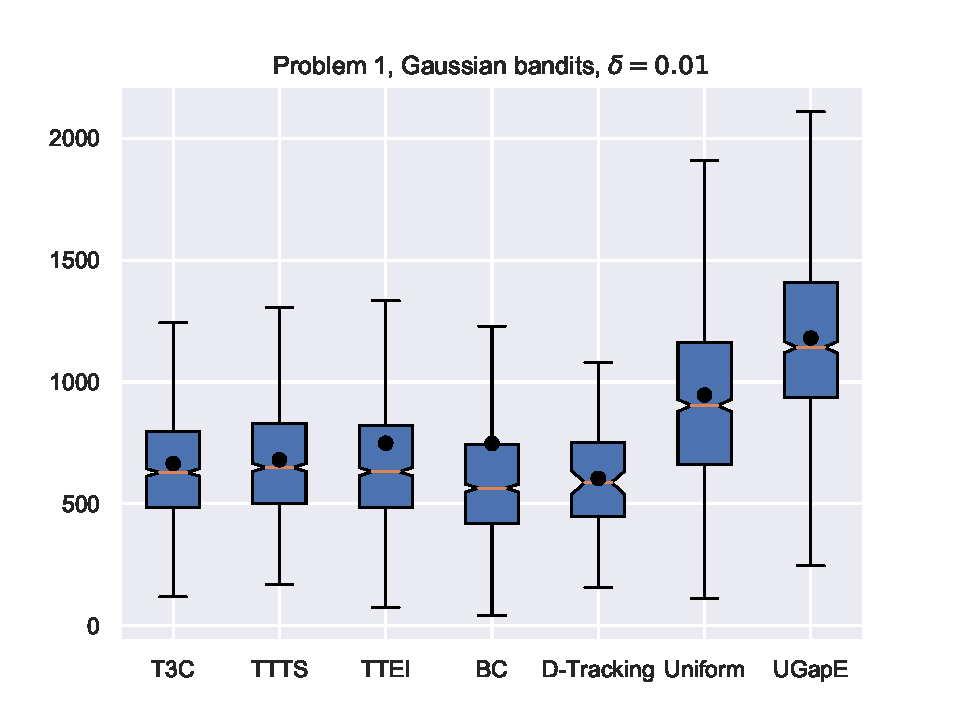
\includegraphics[clip, width= 0.33\textwidth]{Chapter3/img/gaussian1.pdf}
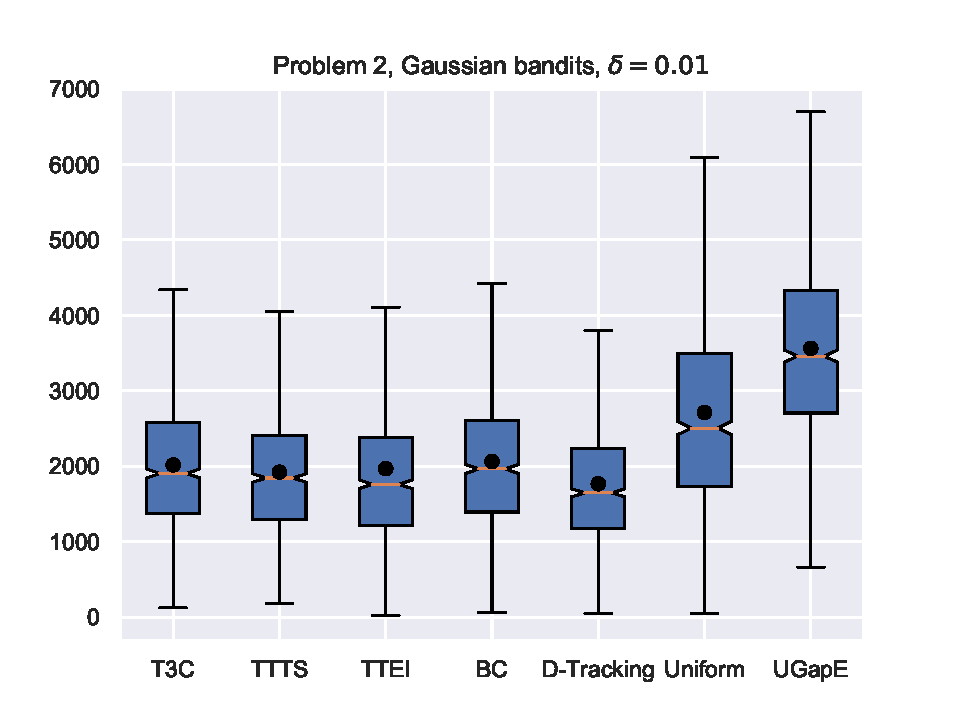
\includegraphics[clip, width= 0.33\textwidth]{Chapter3/img/gaussian2.pdf}
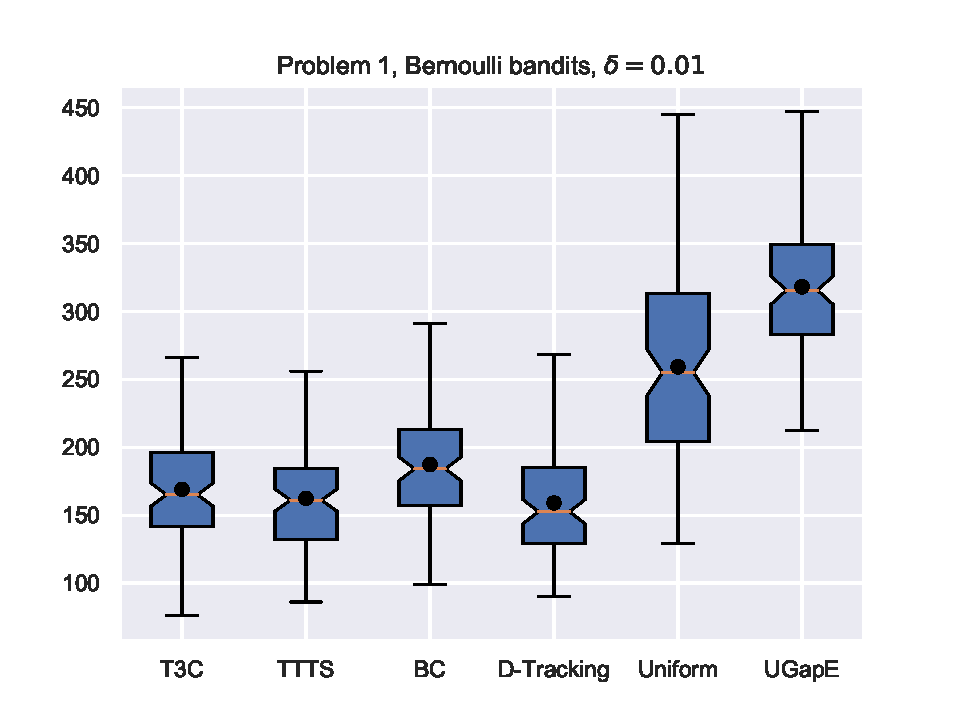
\includegraphics[clip, width= 0.33\textwidth]{Chapter3/img/bernoulli1.pdf}
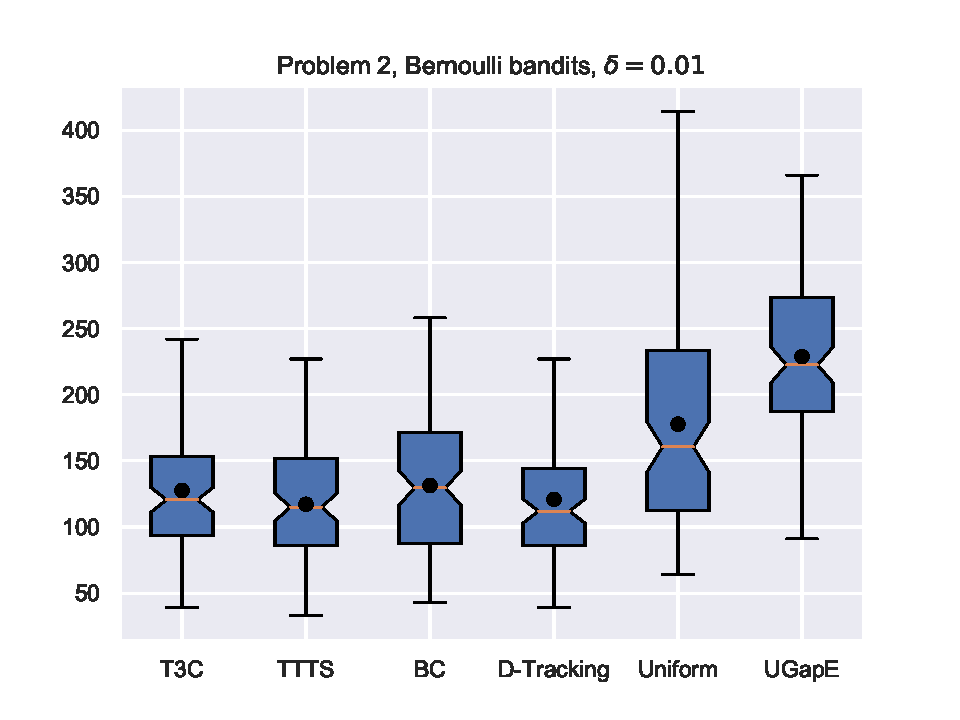
\includegraphics[clip, width= 0.33\textwidth]{Chapter3/img/bernoulli2.pdf}
\caption{Sample complexity of different BAI sampling rules over some random problem instances. Black dots represent means and oranges lines represent medians.}
\label{fig:confidence}
\end{figure*}

These figures provide several insights: (1) \TCC is competitive with, and sometimes slightly better than \TTTS and \TTEI in terms of sample complexity. (2) The \UGapE algorithm has a larger sample complexity than the uniform sampling rule, which highlights the importance of the stopping rule in the fixed-confidence setting. (3) The fact that \DT performs best is not surprising, since it converges to $\bomega^{\beta^\star}$ and achieves minimal sample complexity. However, in terms of computation time, \DT is much worse than other sampling rules, as can be seen in Table~\ref{table:time}, which reports the average execution time of one step of each sampling rule for $\mu_1$ in the Gaussian case. (4) \TTTS also suffers from computational costs, whose origins are explained in Section~\ref{sec:t3c.algorithm}, unlike \TCC and \TTEI. 
Although \TTEI is already computationally more attractive than \TTTS, its practical benefits are limited to the Gaussian case, since the \emph{Expected Improvement} (EI) does not have a closed form beyond this case and its approximation would be costly. In contrast, \TCC can be applied for other distributions.

\begin{table*}[ht]
\centering
\small
%\def\arraystretch{1.2}
\begin{tabular}{|c|c|c|c|c|c|c|c|}
 \hline
 \textbf{Samp. rule} & \TCC & \TTTS & \TTEI & \BC & \texttt{D-T} & \texttt{Uniform} & \UGapE \\
 \hline
 \textbf{Exec. time (s)} & $1.6\times 10^{-5}$ & $2.3\times 10^{-4}$ & $1\times 10^{-5}$ & $1.4\times 10^{-5}$ & $1.3\times 10^{-3}$ & $6\times 10^{-6}$ & $5\times 10^{-6}$ \\
 \hline
\end{tabular}
\caption{Average execution time in seconds for different BAI sampling rules.}
\label{table:time}
\end{table*}
